\chapter{Theoretical Framework}
\label{theoreticalframework}

Language has long played a role in successful advertising. Not surprisingly, as new media have emerged, advertisers have skillfully adapted to form. 

 \cite{Vestergaard:1985vna}  studied the language of press advertisements from 1976--1977. Though noting the contextual role of visual elements, the primary focus of their work was textual.

\begin{quote}
There is no reason to believe that TV and press advertising differ in their persuasive methods in a basic way, although an analysis of TV adverts, owing to the processual character of the TV commercial and its use of both sound and picture, requires an additional body of analytic procedures. \cite[p. 10]{Vestergaard:1985vna}
\end{quote}
\begin{sloppier}
They considered advertising as, fundamentally, a message-based, one-way communication. Though they acknowledged psychological effects of messages, textual content was seen as meaning "transfer".
\end{sloppier}

About the same time,  \cite{Geis:1982uf}  studied linguistic communication in television advertisements. He proposed that advertising discourse was better analyzed under a cooperative model of communication. Commercials both directly address viewers and also communicate indirectly by promoting products through dialogue between characters. He focused strongly on the persuasive use of language, in particular, highlighting the subtle ways in which language can be used to mis-lead consumers.

This chapter presents the notion that some user interactions associated with online behavioral advertising evoke discourse processes using mechanisms similar to those described by  \cite{Geis:1982uf}.  Furthermore, such phenomena are representative of a new sort of advertising discourse. First, I introduce the notion of pragmatics and inferential communication. Then, I describe properties of discourse under a cooperative model. Following this, I discuss the notion of discourse structure and summarize factors contributing to successful communication. Finally, I review two applications of discourse understanding upon which this dissertation builds: graphics communication and the use of language in advertising. 

\section{Pragmatics}
\label{pragmatics}


\begin{quote}
Pragmatics is the systematic study of meaning by virtue of, or dependent on, the use of language. \cite[p. 2]{Huang:2007ww}
\end{quote} 


To understand pragmatics, it's helpful to understand a bit of history in linguistic theory. The study of meaning has long been the domain of semantic theory. Moreover, semantics arose as an extension of philosophical and mathematical logic. In 1905, Bertrand Russell published a short work, ``On Denoting'', in the journal \emph{Mind} which held influence over semantics through much of the 20th century  \citep{Russell:1905tj}.  Russell argued that meaning was propositional and that most statements have truth-value. Such thinking led philosophers to devise a logic-based approach to meaning that forms the basis of formal semantics today.

In a somewhat different vein, J.L. Austin also studied language use in Philosophy. Contrary to Russell,  \cite{Austin:1975vd},  in ``How to Do Things With Words'', argued that the meaning of sentences cannot be characterized solely by truth value. In a theory of speech acts, Austin regarded utterances as performing additional functions. For example, an interrogative cannot have a value of truth or false, but is used to perform an act for the purpose of eliciting some other action (e.g., to obtain information).

\begin{sloppier}
Like Austin, \cite{Grice:1961ud} were also concerned with understanding "non-natural" meaning. They distinguished between two sorts of meaning: the kind of meaning associated with individual words of that utterance (conventional implicature) and what a speaker means by an utterance (conversational implicature). This seems a subtle distinction in the abstract, but is actually an important distinction which had great impact on the discipline now known as pragmatics.
\end{sloppier} 

\textbf{Conventional implicature} relates to the meaning inherent in the words of an utterance. For example, Grice demonstrates using the word ``but'' in the utterance ``she was poor but honest''  \cite[p. 127]{Grice:1961ud}.  What is meant literally, is ``she was poor'' and ``she was honest''. However, ``but'' \emph{implicates} a contrast between ``poor'' and ``honest'', suggesting that honesty is a trait not generally associated with poverty. He notes further that if one were to change ``but'' to ``and'', the literal meaning of the utterance would not change --- but the implication would be gone  \cite[p. 129]{Grice:1961ud}.  

 \cite{Grice:1975vw}  also identified a class of implicatures known as \textbf{conversational implicatures}. This sort of implicature is exemplified by the following example:

\begin{description}
\item Speaker A: Can you close the windows?
\item Speaker B: Sure.
\end{description}

In this example, speaker A is understood by speaker B to be making request. According to Grice, speaker B reasons that speaker A has some reason to make this utterance: it must be somehow relevant to the situation. Conversation implicatures are understood by reference to a \emph{conversational situation} and are inferred via a cooperative principle and general maxims of conversation  \cite[p. 46; covered in more depth later in this chapter]{Grice:1975vw}.  To this end, conversational implicatures also depend on conversants understanding each other's goals and intentions.

In contrast to a formal study of semantics, the discipline of pragmatics holds that the study of language must systematically study meaning \emph{in the context of use}  \citep{Huang:2007ww}.  Under this view, pragmatics is considered a component of an integrated theory of language much as phonetics, phonology, morphology, syntax, and semantics. Phenomena typically considered pragmatic include \textbf{implicature}, \textbf{presupposition}, \textbf{deixis}, and \textbf{speech acts}. 

Presuppositions share some properties of implicature. They are also derived by inference. The famous sentence ``the king of France is bald'' presupposes that there is a king of France, though this is not explicitly stated. Unlike implicature, the presupposition does not change under negation. ``the king of France is not bald'' still presupposes a king of France. 

Deictic expressions are those that make reference to some aspect of context. This context may be expressed symbolically as in ``tomorrow'', ``here'', ``you'', or ``over there'', accompanied by gesture. Deixis is a universal phenomena expressed in all languages. Deixis exists because ``a language without deictics cannot serve the communicative needs of its users as effectively and efficiently as a language which does have them''  \cite[p. 132]{Huang:2007ww}. 

Speech acts derive from Austin's theory of performatives. Under a more general theory of speech acts, speech acts follow certain conventions.  \cite{Searle:1969vw}  defined five types of (illocutionary) speech acts:

\begin{enumerate}
\item \textbf{Assertives} - speech acts which express a proposition with a truth value and play the role of asserting, claiming, reporting, etc.
\item \textbf{Directives} - speech acts which represent an attempt for the speaker to get the addressee to do something as in a question, request, command, etc.
\item \textbf{Commissives} - speech acts which commit the speaker to do something in the future as in a promise, offer, threat, etc.
\item \textbf{Expressives} - speech acts which expresses a psychological state or attitude such as praising, thanking, apologizing, etc.
\item \textbf{Declarations} - speech acts which intend to change bring about change as in a declaration, nomination, etc.
\end{enumerate} 

Functionally, speech acts express strategies for communication. While speech acts have long been considered linguistic acts \cite[][and many others]{Searle:1969vw,Levinson:1983ww}, they also have a social function.\footnote{In fact, \cite{Geis:1995vo} argued that speech acts are not linguistic acts at all --- but social acts. } In standard speech act theory, illocutionary acts are directed toward addressees. \cite{Clark:1982tg} argued, however, that such acts may also be directed toward other participants that are not addressees. Furthermore, they argued that there must be an act called an \textit{informative act} which is directed toward participants who are not addressees. Consider this excerpt from the 1998 movie, \textit{The Truman Show}, where the lead character is unaware that he is starring in a live television drama:
\begin{itemize}
\item [T:] Why do you want to have a baby with me? You can't stand me!
\item [M:] That's not true! ... Why don't you let me fix you some of this Mococoa drink, all natural cocoa beans from the upper slopes of Mount Nicaragua, no artificial sweeteners!
\item [T:] What the hell are you talking about?!? Who are you talking to?!?
\item [M:] I've tasted other cocoas, this is the best!
\end{itemize}
Truman becomes confused because he recognizes that his wife, Meryl, is directing information towards an audience while speaking with him. It's easy to see that participant roles have bearing on how we produce language in interaction. 

One of the great challenges of studying pragmatics is the use of language in social contexts. Of the three experiments in this dissertation, the first concerns the hypothesized incidence of implicature, the second deixis, and the third concerns participant roles in interaction. In Chapter 8, I suggest that these several case studies are potentially indicative that pragmatic reasoning occurs during user interaction online. As we will see, such reasoning may also lead to mis-understanding.
 

\section{Language in Interaction}
\label{languageininteraction}

While philosophy was the well-spring of pragmatics, sociology and anthropology were more concerned with interactional aspects of language. John Gumperz is widely regarded as the ``father'' of interactional sociolinguistics. He and Dell Hymes studied how situations and cultures affect meaning in social interaction  \citep{Gumperz:1982tc,Hymes:1974wr}.  In addition to how words and linguistic expressions affect meaning, they also studied how ``contextualization cues'' in prosody and register (i.e., language used in particular social settings) affect discourse. Gumperz widely influenced the perspective that inferential processes in interaction could be studied systematically in natural communicative contexts. For example, he gives examples of how microinteractions, such as the timing of prosodic and nonverbal cues, give evidence of breakdowns in conversational coordination  \citep{Gumperz:1982tc}. 

Both Gumperz and Hymes strongly referenced pioneering work of Sacks, Schegloff, and Jefferson  \citep{Schegloff:1973tg,Sacks:1974uy,Schegloff:1977tc,Jefferson:1972ta}.  This body of work itself was inspired by the work of sociologist Harold Garfinkel, who was concerned with how activities and routines in daily life inform social interaction.  \cite{Garfinkel:1967vn}  describes research conducted in the 1960s at the Los Angeles Suicide Prevention Center (SPC) and UCLA Outpatient Clinic. He asked the question, ``by what criteria are its applicants selected for treatment?''  \citep[p. 18]{Garfinkel:1967vn}.  Garfinkel's work directly inspired Sacks, Schegloff, and Jefferson to engage in a detailed analysis of conversation which revealed basic organizational features of conversation  \citep{Sacks:1974uy}.  

Their basic insight was that speakers organize contributions in discrete units analyzed as turns. Turns themselves are organized into sequences. According to Sacks, each turn adds to the context affecting what will be done or said in the next turn. Speaker's orient toward each other's turns revealing systematic processes regulating both speech acts contributions as well as mechanisms for error detection and repair  \citep{Levinson:1983ww}.  Pioneering work in conversation analysis in the tradition of ethnomethodology led to deeper understanding of how people manage conversation in interaction and how this system for management helps us to recognize error and repair it when detected. 

 \cite*{Sacks:1974uy}  suggested that ``rules'' (what we now think of patterns) governing the organization of dialogue form the basis of how people manage conversation. For example, short silences or overlap in speech affect how the next speaker in a conversation is selected. Also, prosodic and gestural cues serve as signals during the coordination of exchanges. In addition, structural features such as turn transitions play a role in the detection of error and constrains repairs in dialogue. And repair sequences themselves respect the turn-taking system  \citep{Schegloff:1977tc}. 

Herb Clark, noted cognitive psychologist from Stanford University, studies cognitive and social processes in language use. Building off sociolinguistic theory  \citep{Schegloff:1973tg,Sacks:1974uy,Clark:1989ur,Schegloff:1977tc,Jefferson:1972ta},   he developed a theory of conversation as joint action\footnote{ \begin{quote} 
Clark on Joint Acts: Conversations reflect the joint activities they coordinate. Every joint activity has participants --- the people actually taking part, who are distinct from nonparticipants (bystanders, onlookers, overhearers) --- and so do the conversations that emerge from them. The participants take particular roles, such as doctor and patient, teacher and student, or friend calling and friend called, and the roles constrain what the participants do and say. Every joint activity has public goals --- mutually agreed-upon purposes for carrying them out. The overall goal may be to exchange gossip, plan an outing, or negotiate a contract, and these have subgoals. Although some of these goals are set from the start, most get established as the participants go along. The participants also have private goal --- to be polite, not to lose face, or to finish quickly, for example --- and these, too, constrain what the participants do and say. Finally, people often engage in two or more joint activities at a time --- such as gossiping and eating dinner together --- so their conversation switches back and forth between them. \citeyearpar[p. 2744]{Clark:2001uu}
\end{quote} }  \citep{Clark:2001uu}. \cite{Clark:1989ur}  observed that basic turn construction units patterned into larger chunks of discourse they termed ``contributions''. These units are composed of a distinct presentation phase followed by an acceptance phase. Contributions form a hierarchy where every signal presented (verbal or non-verbal) belongs to the presentation phase of a contribution.

In this example from Clark, the presentation of ``how much does Norman get off -- '' ends with ``oh''.

\begin{description}
\item[Presentation Phase] \hfill \\
A. is it, how much does Norman get off --
\item[Acceptance Phase]  \hfill \\
B. pardon \\
A. how much does Norman get off \\
B. oh
\end{description}

Clark noted that the acceptance phase, generally initiated by B, offers A positive evidence that he understands by what A meant. This could be a verbal response or demonstration of some sort. When B has difficulty understanding, the acceptance phase may become prolonged.

\begin{sloppier}
\cite{Clark:1989ur} posited abstract levels of communication based on patterns of contributions. While a contribution is closed with acceptance, evidence of understanding has the properties of "upward completion" and "downward evidence". For any utterance, B may believe he is in one of four successive states of understanding.
\end{sloppier}
\begin{description}
\item[State 0.] B didn't notice that A uttered something.
\item[State 1.] B noticed that A uttered something  (but wasn't in state 2).
\item[State 2.] B correctly heard the utterance (but wasn't in state 3).
\item[State 3.] B understood what A meant by the utterance.
\end{description}

Understanding in each successive state presupposes understanding in the prior  state (unless evidence from a lower state suggests otherwise).\footnote{\citep{Clark:1996tm} proposed one final state: state 4: B considers taking up A's proposed joint project.} 

The contribution model serves as a means for adding to discourse. However, the amount of evidence required for demonstrating understanding may vary depending on the task. Task-oriented dialogues often require stronger evidence of understanding than other sorts of dialogues  \citep{Clark:1986uw}.  By the principle of least collaborative effort, people ground with as little combined effort as needed for the situation at hand  \citep{Brennan:1996ud}.  

When communicating through a different medium (e.g., phone),  \cite{Clark:2005wk}  predicted that people ground using whatever techniques are available to ground with least collaborative effort. They noted that while a hearer backchannel response such as ``okay'' may be little effort face-to-face or on the phone, it may take considerable effort when teleconferencing or in a chat. The cost of acknowledgement is higher since it may interrupt the speaker.
 
\cite{Clark:1996tm} observed that dialogue gives insight to factors contributing to successful communication.  This includes:
\begin{enumerate}
\item How speakers and listeners cooperate to exchange information;
\item How speakers design utterances to help listeners understand; and,
\item How listeners provide speakers with evidence of understanding.
\end{enumerate}
For conversations to succeed, participants \textbf{ground} what they say: they establish the mutual belief that addressees have understood the speaker well enough for current purposes \citep{Clark:1989ur}. This \textbf{Grounding Hypothesis} suggests information acquired by participants accumulates in a principled way: "each party is responsible for keeping track of what is being said, and for enabling everyone else to keep track of what is being said" \citep{Clark:2001uu}. 
\begin{quote}
With each contribution to the conversation, the current speaker presupposes the common ground already established; and all the parties, the speaker included, add what is new in that contribution to their common ground. \citep[208]{Clark:1992ty}
\end{quote}
Thus, in its broadest interpretation, this view of discourse corresponds to \textit{meaning exchange} using linguistic messages in social and cultural contexts. Importantly, speakers design their utterances taking into account their potential listeners --- listeners themselves are agents in particular roles \citep{Clark:1992ty}.


\section{Discourse}
\label{discourse}

Discourse is a term that is broadly concerned with the use of language. In it's broadest, most functional sense, discourse has been viewed as a kind of social practice  \citep{Goffman:1981tm,Hymes:1974wr,Leech:1983vf,gumperz:1972tf,Brown:1983wy}.  In interactional sociolinguistics, discourse has been studied as ``forms of talk''  \citep{Goffman:1981tm},  characterized as ritualized, or institutionalized talk across social and cultural dimensions. Such talk draws on socio-cultural knowledge governed by social norms which are shared, culturally specific aspects of interpretation  \citep{Gumperz:1982tc,Hymes:1974wr,Gumperz:1964ug}.  Discourse in this perspective is deeply interactive and contextual, acting as a mechanism or process for social exchange.

In conversation analysis, discourse is seen as structured; for example, as interactive frames or schemata such as routinized exchanges in  \cite{Goffman:1981tm}  ``replies and responses'' or  \cite*{Sacks:1974uy}  ``adjacency pairs''. The recognition of such schemata are learned and form the basis for ``co-occurrence expectations''  \citep[p. 162]{Gumperz:1982tc}.  Such conversational inferences are context-bound and conceived as preferences, maxims, or tendencies.

Discourse is also the focus of study in text analysis. ``In its most general significance, a text is a sociological event, a semiotic encounter through which the meanings that constitute the social system are exchanged''  \citep[p. 199]{Halliday:1977vj}.  Such study is concerned with phenomena relating meaning and structure beyond the bounds of a simple turn or sentence --- ``stretches of language received to be meaningful, unified, and purposive''  \citep[p. 156]{Cook:1989wu}.  This includes textual structures playing a role in cohesion, coherence, narrative, and rhetorical structure; cognitive structures such as theme-rheme, topic-focus, foreground-background, given-new, contrasts; and also, syntactic and semantic structures participating in discourse-level anaphora, presupposition, and tense.

\subsection{Discourse Continuum}
\label{discoursecontinuum}

Discourse analysis widely includes practices listed above --- interactional sociolinguistics, conversation analysis, text analysis, and pragmatics. From a cognitive perspective,  \cite{Clark:1996tm}  considers language as a form of \textbf{joint action} embodying individual and social processes. The use of language in joint activities lies on what he calls a \emph{discourse continuum}  \citep[\ref{continuum}][p. 50]{Clark:1996tm}.  


\begin{figure}
\centerline{
  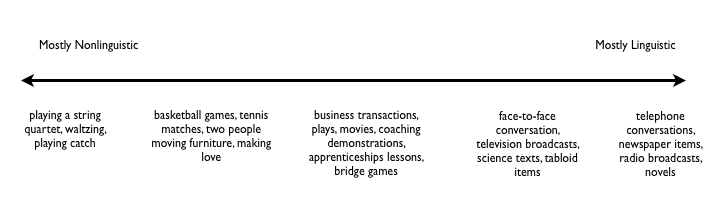
\includegraphics[scale=.75]{chapter3.tex/discourse-continuum}
  }
\caption{Discourse Continuum \citep[adapted from][]{Clark:1996tm}}
\label{continuum}
\end{figure}


To the far right, all activity is accomplished using language. Moving to the left, language is augmented by diagrams, gesture, video etc. In the middle, language is balanced by action, while further to the left, language has less of a role in the content and coordination of activity. But, according to Clark, \textbf{``if we include any signal --- any communicative act --- then language use is present across the entire discourse continuum''}   \citep[p. 51]{Clark:1996tm}.  

In this dissertation, \emph{I claim that user interface components, to include interactive graphics, can be considered as units of discourse} falling somewhat on the right side of of this scale. Undoubtedly, such components contain both graphical and textual elements, but they are also interactive, and as such, trigger patterns of thought and behavior associated with language use. Though such interaction is not strictly conversation --- since applications do not have beliefs and intentions operating in coordination with the user --- application designers model user tasks relying on the user's basic linguistic competence to interpret cues during interaction. This idea will be discussed further Chapter 8.

\subsection{Discourse Models}
\label{discoursemodels}

Ultimately, underlying language use are speaker intentions. Such intentions account for why someone can express the same concept in different ways. For example,  \cite{Donnellan:1966uv}  gave the famous example, ``Smith's murderer was insane'' as an attributive description versus referential description (e.g., ``Jones''). In his view, to say ``Smith's murderer'' is to say something about this person rather than to pick out or identify  him.\footnote{\cite{Kripke:1979ti} distinguished between these two descriptions as contrasting a semantic referent with a speaker referent.} 

But this sort of indefinite reference raises problems for a semantic analysis of reference. To account for a range of discourse phenomena such as this,  \cite{Kamp:1993wm}  proposed a theory of discourse representation which includes a representation of a \textbf{discourse model}. This structure contains a set of discourse referents (entities under discussion) and conditions which represent information that has been given about referents.

 \cite{Kamp:1993wm}  and, independently  \cite{Heim:1982wp},  made it possible to analyze chunks of discourse using a semantic analysis. But the idea of discourse models was not entirely new. ``Discourse models make explicit the structure of not of sentences but of situations as we perceive and imagine them''  \cite[p. 419]{JohnsonLaird:1983vt}.  Such models help to account for how people comprehend language. One piece of evidence given for discourse models are \textbf{bridging inferences} --- a sort of implicature by which people flesh out missing details in discourse  \citep{Clark:2002vz}. \cite{Stenning:2008uh} and \cite{JohnsonLaird:1989uj}  cited work from  \cite*{Bransford:1972tz}  giving experimental evidence that recalled sentences are inferences from explicitly presented material. An example used was,

\begin{itemize}
\item[(a)] Three turtles rested on a floating log and a fish swam beneath them.
\end{itemize}
Subject later confused this sentence with:
\begin{itemize}
\item[(b)] Three turtles rested on a floating log and a fish swam beneath it. 
\end{itemize}

 \cite{Bransford:1972tz}  argued that memory for language draws on the use of representations organized around referents (entities) in scenes and events. Models are updated incrementally and inferences about participants are made when needed. In this way, its possible to remember things about a discourse referent while not remembering how the information was conveyed.

The notion of direct and indirect representations made by  \cite{Stenning:1995ka}  is important. In their view, while indirect representations such as those used in language have a syntax, direct representations do not. It is the aim of a discourse model to provide a direct representation. As discourse proceeds, the discourse model is revised to accommodate new beliefs, but is also subject to revision when conflicting information arises. The notion of a discourse model has been crucial to theory in linguistics that accommodates a wide range of semantic-pragmatic phenomena to include anaphora, deixis, tense, and presupposition. Discourse models have also been applied to graphical reasoning where such representations are posited as a means to achieve efficiency in cognitive processing given constraints in working memory  \citep{Stenning:1995ka}. 

Discourse models have been formalized in semantics  \citep{Kamp:1993wm},  computational linguistics and artificial intelligence  \citep{Hobbs:1985ue,Grosz:1989wu},  cognitive science  \citep{Stenning:2002vd,JohnsonLaird:1989uj,vanDijk:1983tk}  and cognitive psychology  \citep{Clark:1996tm}.  In these models, discourse is structured to account for informational links as well as the role of context in meaning  \citep{Grosz:1986up}.  Discourse is also considered fundamentally cooperative, thus models take into account belief and attentional states of addressees  \citep{Clark:1996tm}.  Finally, such models account for the role of lexical, grammatical, and structural properties of language in pragmatic inference.

Thus, \emph{discourse processes concern how information is comprehended and produced}. This involves creating, accessing, and using discourse representations (or models)  \citep{Graesser:2012wz}. As \cite*{Graesser:2012wz}  observed, discourse processing research is multi-disciplinary encompassing linguistics, psychology, computer science, and neuroscience. Techniques used in study include corpus analysis, mathematical and statistical modeling, ``on-line'' experimentation (e.g., during comprehension), and brain imaging. 

While discourse researchers have busily been studying new forms of communication --- some broadcast-oriented, such as lectures, radio \slash  podcast, print advertising --- others more interactive, such as those found in computer-mediated discourse (e.g., discussion forums, chat, microblogging, and blogging), little attention has been yet afforded to direct interaction with media such as multimedia advertisements. To do so would necessitate analyzing the coordinated use of both graphics and language. The next section of this chapter specifically looks at work associated with graphics and diagram understanding and the role of discourse models as a unified representation for textual and graphical elements.

\section{Applications}
\label{applications}

In this section, I consider two applications of discourse understanding relevant to claims made in this dissertation: graphics communication and advertising language. The first summarizes work claiming that implicatures may be understood in graphical diagrams. The second describes how advertisers make use of language to persuade and manipulate. Both are relevant to a discussion of how people may be manipulated in user interaction in the context of online behavioral advertising.

\subsection{Graphics Communication}
\label{graphicscommunication}

There is reason to think that messages produced by graphical user interfaces may be interpreted under the same inferential model of communication as language.  \cite{Stenning:2006wu}  define graphics as ``planar displays of information that use the distribution of shapes, patterns, and annotations and the relation between them to convey information''  \cite[p. 476]{Stenning:2006wu}.  In simpler terms, graphics use spatial relations, in addition to text labels, to convey meaning. Good examples are maps, tables, and charts. 

 \cite{Stenning:2006wu}  note that their definition also fits textual language. While text on a page is essentially organized linearly, there is an abstract syntactic structure which encodes meaning relations between parts -- thus mapping to space indirectly. Graphics, on the other hand, encode meaning in a direct spatial representation. 

Diagrams are limited in the number of dimensions they can use to map relations. This might include icon shape, color, order, etc. Each dimension is directly mapped to a semantic representation. Phrases, words, morphemes, and phonemes, on the other hand, pack many relations across multiple abstract levels, each syntactic relation having a distinct semantic representation.

 \cite{Tversky:2004wj,Tversky:2010ww}  summarized a body of psychological experimentation demonstrating parallels between graphics, gesture, and language. Shared cognitive principles allow for mapping between visual and verbal modes in a number of domains. She described work from  \cite{Denis:1997}  in which route directions and maps could both be decomposed into a series of segments. Each segment was described to have four elements: a start point, orientation, progression, and end point. For example, ``exit the Central Square station, turn left, go down Mass Avenue until you come to Cafe Centro''  \cite[p. 146]{Tversky:2004wj}.  The correspondence between both descriptive textual elements and graphical depictive elements suggest a common, underlying conceptual structure.

Tversky argued that such meanings of schematic visual forms (glyphs and other devices) both convey and constrain meaning  \cite{Tversky:2010ww}.  Glyphs combine into complex diagrams using domain-specific syntax rules in a manner similar to linguistic structures  \citep{Tversky:1999ta}.  Similarly,  \cite{Tversky:2010ww}  noted that glyphs may be used to abstractly represent a variety of concepts such as objects, collections, relations, and processes. Such representations participate in cognitive processes such as ``inference, analogy, generalization, transfer, and insight''  \citep[p. 2]{Tversky:2010ww}. 

Though graphics and language differ in expressiveness and information packaging, they can both be studied using pragmatic theory  \citep{Stenning:2002vd,Stenning:1995ka}. \cite{JohnsonLaird:1989uj}  described the machinery by which linguistic representations (logical syllogisms expressed graphically) can be used to construct and update a  mental model\footnote{Mental models are considered equivalent to discourse models \citep{JohnsonLaird:1980uf}. However, the term "discourse model" is preferred here as it is has been more widely adopted by researchers in the academic traditions discussed.}. 

A syllogism consists of two premises followed by a conclusion as in:

\begin{enumerate}
\item All A are B
\item All B are C
\item Therefore, all A are C
\end{enumerate}

Syllogisms are defined from a narrow set of ``moods'': All A are B, No A are B, Some A are not B  \citep{Khemlani:2012ii}.  It is also possible to make constructions that look like syllogisms such as:

\begin{enumerate}
\item In some cases when I go out, I am not in company.
\item Every time I am very happy I am in company.
\item Therefore, in some cases when I go out, I am not very happy. \cite[p. 1]{Khemlani:2012ii}
\end{enumerate}

What makes example above different is the application of \emph{quantifiers} (e.g., more than) and \emph{determiners} (all, every, some, etc.) and over more complex objects such as sets and events. Contrast this with the limited logic of ``all'', ``some'', and ``no'' in a syllogism. The construction seems very similar --- but its meaning potentially much more complex.

Such constructions are interesting to study because they are informative of how people reason and also amenable to online (realtime) experimentation. Interestingly, not only does content affect reasoning (e.g., people are more likely to accept a believable conclusion than unbelievable) but when encountering such constructions, people are also highly susceptible to pragmatic inference  \citep{Khemlani:2012ii}.  

Another interesting property is that they can be expressed graphically. In fact, such graphics are effective methods for teaching deductive logic  \citep{Stenning:1995ka}.  Euler diagrams, such as  \autoref{euler}  helps aid comprehension by providing a more direct representation of the syllogism at the top of this section.


\begin{figure}
\centerline{
  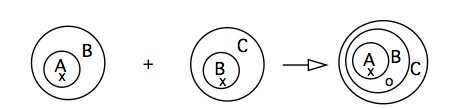
\includegraphics[scale=.75]{chapter3.tex/syllogism}
  }
\caption{Graphical Syllogism \citep{Stenning:1995ka}}
\label{euler}
\end{figure}


 \cite{JohnsonLaird:2007ua}  argued that, in fact, people do not learn as children a ``mental logic''. They acquire understanding of lexical structures (including connectives, quantifiers, relation terms, etc.) and use these to construct models of premises. Inferential schemas and the ability to calculate semantic validity are what's necessary for logical reasoning.

While  \cite{Oberlander:1995vv}  argued for graphical implicature in the use of graphical notations for computer-assisted design in electronics, I argue that implicature can also be found in user interfaces. This makes them particularly amenable for deliberate manipulation. The next section focuses on how advertisers use language to persuade and manipulate. The use of graphics and language for advertising have been a rich area of study, though not yet in the context of interaction.

\subsection{Advertising and Language}
\label{advertisingandlanguage}


\cite{Cook:2001up} argued that advertising is, in itself, a form of discourse.  Though previous linguistic analysis tackled such discourse by focusing primarily on textual or verbal elements, he argues that other contextual elements should not be divorced from analysis.  This is in contrast to earlier attempts to study language use in advertising where linguistic analysis had focused primarily on textual content and style \citep{Leech:1966wr,Vestergaard:1985vna}.

As \cite{Geis:1982uf} observed in his study of the language of television advertising,\footnote{Geis's \citeyearpar{Geis:1982uf} study is based on the analysis of 800 commercials made between 1978 and 1981.} the goal of commercial advertising is to get consumers to buy. \cite{Geis:1982uf} focuses especially on the arguments that advertisers use in order to persuade users to buy products. By persuasion, Geis meant the process by which a message is taken up such that the recipient is convinced of its truth or is moved to act. He distinguished this from manipulation in that \textit{persuasion involves conscious evaluation by the recipient on the source message and manipulation does not}.

Not surprisingly, language can and does play an important role in the process of persuasive advertising. Advertisers use language to convey messages, but also for more subtle purposes. As Geis noted, language performs a role in getting viewer attention, supporting arguments used to persuade, and playing a role in facilitating consumer memory on the desirability of the product or service \cite[p. 23]{Geis:1982uf}.

Central to how advertisers use language for persuasion is the notion of implication. Advertisers are bound legally not to use deception in order to sell. \cite{Brandt:2013un} observed that the FTC took a strong position on "misleading advertising" during the 1970s. During this time, it recognized the role of cognitive research in demonstrating how consumer world knowledge might interact with ads to form false beliefs. Thus the FTC began to rely on behavioral research to determine whether an ad was misleading. In fact, there are many ways ads can be misleading without direct assertion. 

\begin{quote}
Probably a fundamental reason has been the more subtle forms of deception that the FTC has become desirous of controlling. 'Was it deceptive for Wonder Bread (ITT, 1973) to claim it is high in nutrition when the claim is literally true yet might imply falsely that the quality is unique to itself? Did the name "Safety Champion" (Firestone, 19721 Firestone, 1973) imply that a tire is perfectly safe, or that it is safer than other tires? \citep[p. 5]{Brandt:2013un}
\end{quote}

\subsubsection{Persuasion Through Implicature}
Geis adopted a Gricean position on advertising precisely because advertisers often persuade through the use of implicatures. He gives the following example,
\begin{itemize}
\item[(a)] Wartsoff contains Vivaline and you know that Vivaline removes warts instantly. \citep[p. 26]{Geis:1982uf}
\end{itemize}
The implication is that Wartsoff removes warts instantly. An unsuspecting consumer might reason that since the advertiser used the verb "know", there must be solid evidence that Vivaline removes warts instantly.

Geis focused on three sorts of implicatures: 1) conventional implicatures; 2) theoretical implicatures (those which depend on listener belief for validity); and, 3) conversational implicatures.  

The Wartsoff statement is an example of a conventional (embedded) implicature by the use of "know". Because the word "know" has been used, it is implicated that there is good evidence supporting that Vivaline removes warts instantly.

A theoretical implicature, on the other hand, is given by the example:
\begin{itemize}
\item[(b)] Choosy mothers choose Jif. \citep[p. 48]{Geis:1982uf}
\end{itemize}
The implication is that if a mother doesn't choose Jif, she isn't a good mother.

Finally, the following is an example of a conversation implicatures:
\begin{itemize}
\item[(c)] We're building a reputation, not resting on one. \citep[p. 50]{Geis:1982uf} citing an ad in Newsweek, 2/6/1978
\end{itemize}

Here the implication is that Ramada Inn has a leading competitor that rests on its reputation. But, of course, this is not explicitly said. However, because resting on a reputation was mentioned --- it must in some way be relevant to the listener.

To back off just a bit, \cite{Grice:1975vz} proposed that language is governed by the Cooperative Principle. According to Grice, the cooperative use of language in conversation appears to follow certain maxims, or rules. In particular,

\begin{description}
\item \textbf{Quantity:} Say no more and no less than is necessary.
\item \textbf{Quality:} Say what you believe to be true; do not say what lacks adequate evidence.
\item \textbf{Relation:} Say what is appropriate at the appropriate time; be relevant.
\item \textbf{Manner:} Be clear; be brief; be perspicuous; avoid obscure expressions.
\end{description}

Grice hypothesized that such maxims generate implicatures. In particular, he focused on examples of when such maxims were "flouted" such that the listener is expected to understand the message, despite violation of  conversational rules.

In fact, we flout these maxims on a regular basis. Examples of obvious flouting are in the use of irony and metaphor. 
\begin{itemize}
\item[(d)] Brilliant! (Exclaimed after tripping)
\item[(e)] Great weather we're having. (After sudden clap of thunder)
\item[(f)] Those two are peas in a pod.
\end{itemize}
\cite{Tanaka:1999tq} noted the use of metaphors and puns in advertisement.
\begin{itemize}
\item[(g)] What makes a shy girl get Intimate (Intimate, Revlon) \citep[p.104]{Tanaka:1999tq}
\end{itemize}
She suggested that the reader is expected to get and reject:
\begin{itemize}
\item[(h)] What makes a shy girl become intimate.
\end{itemize}
in favor of:
\begin{itemize}
\item[(i)] What makes a shy girl buy Intimate perfume.
\end{itemize}
Likely, such use of implicature is intended to attract attention and intrigue and not to mislead. 

\cite{Geis:1982uf} argued that while advertisers may be held accountable for misleading the public through conventional and theoretical implicature, this may not the case for conversational implicature.
\begin{itemize}
\item[(j)] Wet feet? LOOK OUT FOR A COLD --- Gargle with LISTERINE QUICK \cite[p. 49]{Geis:1982uf}
\end{itemize}
In the example above, attributed to \cite{clark1944advertising}, Listerine is conversationally implicated by the Maxim of Relevance. In fact, Geis mentions that after 40 years of advertising in this manner, the advertisers was finally compelled by the FTC to add the disclaimer:

\begin{quote}
While Listerine will not help prevent colds or sore throats or lessen their severity, Listerine's strong formula keeps your breath clean for hours --- it kills the germs that can cause bad breath.
\end{quote}

In this disclaimer, the advertiser still exploits a conventional implication by stating that Listerine does not help prevent colds. As Geis notes, conventional implicatures are perceptually less salient than assertions though, nonetheless, implicate a relation.


 \subsubsection{Overt and Covert Communication} 

 \cite{Sperber:1986uk}  argued that there is reason to recognize a distinction between an \emph{informative intention} and \emph{communicative intention}. The first makes ``manifest or more manifest to the audience a set of assumptions.''  \citep[p. 58]{Sperber:1986uk}  The second makes it `` mutually manifest to audience and communicator that the communicator has this informative intention.''  \citep[p. 61]{Sperber:1986uk} 

\begin{sloppier}
In \textbf{ostensive-inferential communication}, as described by \cite{Sperber:1986uk}, an ostensive act by the communicator is intended to be recognized. Thus, a pointing gesture intends to draw attention to some aspect of the physical context that the communicator thinks worthy of attention. 
\end{sloppier}

In  \cite{Sperber:1986uk}  view, \textbf{relevance} is the key to human cognition. Humans pay attention to things most relevant. A communicator that \emph{manipulates context} has an affect over what is perceived more or less relevant. This means that the communicator needs to be aware of what contextual information is accessible to the addressee in order affect the process of comprehension.

From this point-of-view, ostensive communication is successful if the hearer is able to ``recover the speaker's informative intention''. \textbf{Covert communication}, on the other hand, is described as:

\begin{quote}
A case of communication where the intention of the speaker is to alter the cognitive environment of the hearer, i.e., to make a set of assumptions more manifest to her, without making this intuition mutually manifest. \citep[as quoted in Tanaka 1994, p. 41]{Bencherif:1987up}
\end{quote}

 \cite{Tanaka:1999tq}  argued that covert communication is used in advertising for two main purposes. First, to make the addressee forget that he is trying to sell her something. Second, to ``avoid taking responsibility for the social consequences of certain implications arising from advertisements''  \citep[p. 44]{Tanaka:1999tq}.  Tanaka follows with a number of examples centered on the use of sexual imagery and captioning to promote products which are not obviously sexual. For example, she shows an image from a watch ad where there is a background image of a man and woman in swimsuits embracing. A subtle caption indicates: ``designed to perform.'' Though the ad overtly communicates that these watches are designed to perform well in aquatic sports, there are strong suggestive overtones in the image clearly implicating sexual performance.

As  \cite{Sperber:1986uk}  noted, a large difference between Grice's approach (to include neo-Gricean theories proposed by  \citealp{Horn:2006va} and \citealp{Levinson:2000ud})  and theirs  (i.e., \textbf{Relevance Theory})  is that Grice's principle and maxims are norms that all people are expected to know and recognize. Implicatures are recognized and understood as violation of these known norms. By contrast, Relevance Theory is general to the point that people don't need to recognize or know anything. All that is necessary is that each ostensively communicated act have a presumption of relevance.

As advertising has adapted to new forms of media, so has the means by which advertisers harness language. Though researchers have made study of press and television advertising, little attention has been paid to behavioral and interactive advertising (with the exception of privacy notices). One can already imagine ads where people who look like one's friends recommend products used by those friends. More subtle are ad interactions, hidden in plain sight, that alter one's beliefs in fleeting moments in time. It would not be surprising to find that advertisers exploit cognitive tendencies in inferential communication activated during the course interaction.

\section{Conclusion}
\label{conclusion}

On the basis of reviewed literature, I propose that there are gaps in knowledge that have not yet been addressed: first, that interaction with graphical user interfaces involve discourse processes affecting comprehension; and second, that online behavioral advertising participates in a new form of advertising discourse where user's beliefs are affected during the course of interaction. I show that this view gives insight into communication errors difficult to explain otherwise.

\begin{sloppier}
The next chapter describes my research program and method for data collection and analysis. To follow in Chapters 5 through 7, I focus on specific sorts of pragmatic mis-understandings in the domain of online behavioral advertising.  Each time a user opens a web browser and interacts with a website, that user is challenged to make decisions about what to communicate --- and to whom --- in an environment where commercial actors actively encourage disclosure. Because discourse comprehension relies much on inference, manipulation may subtly take advantage of automatic processes such that the user is unaware of the potential for mis-understanding. Though \cite{Kahneman:1984td} and others have observed that small changes in context affect judgement and decision-making, there is considerably less research on how small changes in context affect understanding during the course of interaction in decision-making tasks. This is the topic under discussion in the remainder of this dissertation.
\end{sloppier}

